\chapter{Il problema di corrispondenza di post} \label{ch:capitolo7}
\subsection{PCP}
Un’istanza del problema di corrispondenza di Post (PCP)è una ($2$n)-pla di parole:
\begin{center}
    ($u_1, v_1; u_2, v_2;...;u_n,v_n$)
\end{center}
Su un alfabeto A, $n >= 1$.\\
Un match di tale istanza è una sequenza $i_1, i_2,...,i_k$ con$ k > 0$, tale che
\begin{center}
    $u_{i1},u_{i2} ... u_{ik} = v_{i1},v_{i2} ... v_{ik}$
\end{center}
Denotiamo con PCP l’insieme delle istanze che hanno un match.\\\\
\textbf{Osservazione}\\
In termini algebrici, PCP è l’insieme delle coppie di omomorfismi di semigruppi liberi $g, h : B^+ \mapsto A^+$ che coincidono almeno su una parola di $A^+$.
\newpage
\subsection{Problema corrispondenza di post}
\textbf{Esempio}\\
Consideriamo l’istanza (b,ca;a,ab;ca,a;abc,c) che possiamo rappresentare nella forma
\begin{figure}[htp]
    \centering
    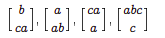
\includegraphics[scale=0.8]{tesi_stile/img/cap7f1.png}
\end{figure}\\
Un match si ottiene concatenando
\begin{figure}[htp]
    \centering
    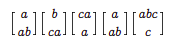
\includegraphics[scale=0.8]{tesi_stile/img/cap7f2.png}
\end{figure}\\
\textbf{Esempio}\\
L’istanza\\
\begin{figure}[htp]
    \centering
    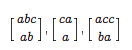
\includegraphics[scale=0.8]{tesi_stile/img/cap7f3.png}
\end{figure}\\
non ha match.\\\\
\textbf{Teorema}\\
PCP è indecidibile.\\\\
\textbf{Dimostrazione}\\
Mostreremo che il problema dell’arresto si riduce a PCP.\\
Consideriamo il seguente problema di corrispondenza di Post modificato:\\\\
\textbf{Definizione}\\
MPCP è l’insieme delle istanze di PCP che hanno un match tale che $i_1 = 1$.\\\\
\textbf{Proposizione}\\
Il problema dell’arresto si riduce a MPCP.
\subsection{Ridurre l'arresto MPCP}
Dobbiamo costruire una funzione che a ogni macchina di Turing M e ogni input w associ un’istanza $P_{M,w}$ di MPCP, in modo tale che M $\downarrow$ w se e solo se $P_{M,w}$ ha un match con $i_1 = 1$.\\
Possiamo ridurci al caso di macchine di Turing che
\begin{itemize}
    \item si arrestano solo in un fissato stato $q_h$
    
    \item ogni volta che entrano nello stato $q_h$ si arrestano
\end{itemize}
Costruiremo un’istanza di MPCP in cui un match riflette, in qualche modo, la computazione di M su w.
\subsection{Costruzione dell'istanza}
Poniamo 
\begin{figure}[htp]
    \centering
    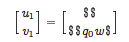
\includegraphics[scale=0.9]{tesi_stile/img/cap7f4.png}
\end{figure}\\
Per ogni quintupla $(q,a,r,b, +1)$ aggiungiamo la coppia\\
\begin{figure}[htp]
    \centering
    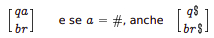
\includegraphics[scale=0.9]{tesi_stile/img/cap7f5.png}
\end{figure}\\
Per ogni quintupla $(q,a,r,b, -1)$ aggiungiamo le coppie\\
\begin{figure}[htp]
    \centering
    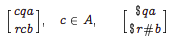
\includegraphics[scale=0.9]{tesi_stile/img/cap7f6.png}
\end{figure}\\
\newpage
Per ogni $a \in A$ U $\{\#,\$\}$, aggiungiamo la coppia\\
\begin{figure}[htp]
    \centering
    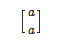
\includegraphics[scale=0.9]{tesi_stile/img/cap7f8.png}
\end{figure}\\
Infine aggiungeremo le coppie\\
\begin{figure}[htp]
    \centering
    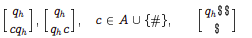
\includegraphics[scale=0.9]{tesi_stile/img/cap7f9.png}
\end{figure}\\
\textbf{Esempio}\\
Istruzioni:
\begin{center}
    $(q_0, 1, q_1, \#, +1), (q_0, \#, q_0, \#, +1), (q_1, 1, q_0, \#, +1), (q_1, \#, q_h , \#, +1)$
\end{center}
Input: w = 111\\
Istanza di MPCP:
\begin{figure}[htp]
    \centering
    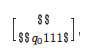
\includegraphics[scale=0.8]{tesi_stile/img/cap7f10.png}
    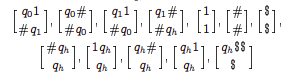
\includegraphics[scale=0.8]{tesi_stile/img/cap7f11.png}
    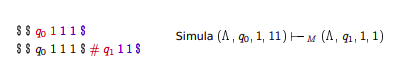
\includegraphics[scale=0.8]{tesi_stile/img/cap7f12.png}
\end{figure}\\
\begin{center}
    \textbf{Se M $\uparrow$ w non ci sono match !}
\end{center}
\newpage
\subsection{Ridurre MPCP a PCP}
\begin{figure}[htp]
    \centering
    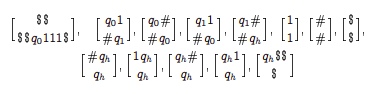
\includegraphics[scale=0.9]{tesi_stile/img/cap7f13.png}
\end{figure}
Se invece M $\downarrow$ w, continuando, otterremo\\
\begin{figure}[htp]
    \centering
    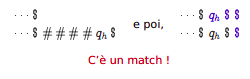
\includegraphics[scale=0.9]{tesi_stile/img/cap7f14.png}
\end{figure}\\
\textbf{Asserto}\\
Si ha M $\downarrow$ w se e solo se $P_{M,w} \in$ MPCP.\\\\
\textbf{Corollario}\\
Il problema dell’arresto si riduce a MPCP.\\
Ora costruiamo una riduzione di MPCP a PCP. Per ogni parola $w =a_1a_2 ... a_l$, denotiamo:
\begin{center}
    $*w = *a_1 *a_2 ... *a_l$,  $w*=a_1* a_2* ... a_l*$
\end{center}
Dobbiamo costruire una funzione che a ogni istanza P di MPCP associ un'istanza P' di PCP, in modo tale che P ha un match con $i_1 = 1$ se e solo se P' ha un match.\\
Sia $P = (u_1, v_1; u_2, v_2;...;u_n,v_n)$. Definiamo\\
\begin{center}
   P' = $(*u_1,v_1*; *u_1, v_1*;*u_2, v_2*; ... , *u_n, v_n*; *o, o)$
\end{center}
\newpage
\begin{figure}[htp]
    
\includegraphics[scale=0.9]{tesi_stile/img/cap7f16.png}
\end{figure}
Viceversa, se P ha un match con $i_1 = 1$, allora ci sarà anche un match di P'.
Se ne conclude che P' $\in$ PCP se e solo se P $\in$ MPCP.\\\\
\textbf{Conclusione}\\
Abbiamo costruito una riduzione del problema dell’arresto a MPCP e una riduzione di MPCP a PCP.\\
Poichè il problema dell’arresto è indecidibile, lo sono anche MPCP e PCP.
\subsection{Matrici con angolo zero in alto a destra}
\textbf{Problema (Zero nell’angolo)}\\
Dato un insieme finito M di matrici 3 x 3 a coefficienti interi, esiste un prodotto di matrici di M che ha uno 0 nell’angolo in alto a destra?.\\\\
\textbf{Teorema}\\
Il problema Zero nell’angolo è indecidibile.\\\\
\textbf{Dimostrazione}\\
PCP si riduce al problema Zero nell’angolo.
\newpage
\subsection{Riduzione di PCP a Zero nell’angolo}
Sia $P = (u_1,v_1;...;u_n,v_n)$ un’istanza di PCP.\\
Costruiremo un insieme di matrici M = $\{M_1,.., M_n\}$ tali che P $\in$ PCP.\\
se e solo se M contiene una matrice con zero nell’angolo in alto a destra. \\
Possiamo supporre, senza perdita di generalità, che l’alfabeto sia $\{1, 2, . . . , d - 1\}$.\\
Per $i=1, . . . , n$ definiamo:
\begin{figure}[htp]
    \centering
    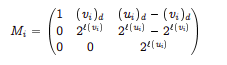
\includegraphics[scale=0.9]{tesi_stile/img/cap7f17.png}
\end{figure}\\
dove $(w)_d$ è il numero denotato da w in base d. Si verifica facilmente che
\begin{figure}[htp]
    \centering
    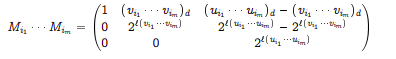
\includegraphics[scale=0.9]{tesi_stile/img/cap7f18.png}
\end{figure}\\
$i_1, . . . , i_m \in \{1, . . . , n\}$.\\
Ma allora $M_{i1}...M_{im}$ ha zero nell’angolo in alto a destra se e solo se $(i_1, . . . , i_m )$ è un match di P.\\
Questo prova che la funzione $P \mapsto M$ è una riduzione di PCP a Zero nell’angolo.\\
Con tecniche simili, si dimostra l’indecidibilità del \textbf{problema di mortalità} per le matrici 3 x 3 a coefficienti interi:\\\\
\textbf{Problema (mortalità)}\\
Dato un insieme finito M di matrici 3 x 3 a coefficienti interi, esiste un prodotto di matrici di M uguale alla matrice nulla?
\newpage
\subsection{CFG ambigue}
\textbf{Definizione}\\
Una grammatica non contestuale è ambigua se esiste una parola con due derivazioni sinistre.\\\\
\textbf{Teorema}\\
È indecidibile se una grammatica non contestuale è ambigua.\\\\
\textbf{Dimostrazione}\\
PCP si riduce all’ambiguità delle grammatiche non contestuali.\\
Sia $P = (u_1,v_1; . . . ;u_n,v_n)$ un’istanza di PCP.\\
Costruiremo una grammatica non contestuale G che è ambigua se e solo se P $\in$ PCP.\\
Siano c1,..., cn n nuove lettere e G la grammatica con le produzioni\\
\begin{center}
    $ S \mapsto X$ | $Y, X \mapsto u_iX_{ci}$ | $uici, Y \mapsto v_iY_{ci}$ | $vici$, i = 1, . . . , n.
\end{center}
Si verifica facilmente che G genera il linguaggio:
\begin{figure}[htp]
    \centering
    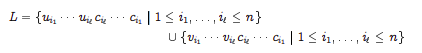
\includegraphics[scale=0.9]{tesi_stile/img/cap7f20.png}
\end{figure}
Non è poi difficile convincersi che G è ambigua se e soltanto se
\begin{center}
    $u_{i1} ... u_{il} = v_{i1} ... v_{il}$
\end{center}
per opportuni $i_1, . . . , i_l$ cioè se e soltanto se P ha un match.